\documentclass[article, 1.5space, letterpaper, 12pt, oneside, header, footer]{SydeClass}
\graphicspath{{images/}}
\usepackage{subfigure}
\usepackage{amsmath}
\usepackage{eqnarray}
\usepackage{rotating}

\usepackage{array}
\usepackage{multirow}




% --------- Title Info -----------
\titlestyle{design} % used in SydeTitle.tex. Can equal one of the following values: design, work

\title{Lab 1}
\subtitle{Clusters and Classification Boundaries}

\coursecode{SYDE 372}
\department{Systems Design Engineering}

\author{Colin Heics, 20240543}
\authorheader{C. Heics}
\authortwo{Rob Sparrow, 20275155}
\authorheadertwo{R. Sparrow}
\authorthree{Philip Wang, 20276999}
\authorheaderthree{P. Wang}

\date{\today}
\instructor{Alex Wong}

\subsectionfont{\normalsize}
\setcounter{secnumdepth}{2}
\setcounter{tocdepth}{1}

\input{matlabFormating}

% ############  ############
\begin{document}

% ---------- Title ------------
\input{SydeTitle}

% ############ Chapters ############
\pagenumbering{arabic}

\section{Introduction}
This lab investigates three areas: calculating orthonormal transformations, creating decision boundaries using different classification methods, and assessing classification error associated with different methods. All calculations for the purpose of this lab are carried out using the MATLAB program.

First, data for five separate classes is generated using bivariate Gaussian distribution parameters provided in the lab description. This results in five clusters of two-dimensional data being generated, based on the underlying statistics specified, which is analyzed with respect to the unit standard deviation contour in each class. Analysis of the data is separated into two cases: Case 1 corresponding to the first two classes, and Case 2 corresponding to the remaining three.

Next, five separate classification methods are developed to allow for the plotting of decision boundaries in each of the two cases. First, the Mean Euclidean Distance (MED), Generalized Euclidean Distance (GED), and Maximum A Posteriori (MAP) methods are implemented and applied to all classes of data. Decision boundaries are plotted for all three methods using data from each of the cases developed previously, to allow for qualitative comparison of the boundaries. Next, the Nearest Neighbor (NN) and Five Nearest Neighbor (5NN) methods are applied to all classes of data. The decision boundaries for both methods are plotted again for the Case 1 and Case 2 sets of classes to allow for comparison.

Lastly, the experimental error rate and confusion matrices are developed for each method applied to both Case 1 and Case 2. The experimental error and confusion matrices are analyzed to allow for comparison between the experimental results of each method. 

\section{Generating Clusters}
Clusters were generated by sampling from a Gaussian distribution, then transforming the samples of each cluster based on the cluster's mean and covariance matrix. The random samples of a standard two-variable Gaussian distribution were generated using MATLAB's $randn()$ function. The samples were then transformed as shown by the example in MATLAB's documentation for $randn()$. The example shows to transform a given vector, x, by the equation
\begin{eqnarray}
\label{eqn:chol_transform}
\underbar{y} = chol \Sigma \underbar{x}+\underbar{\mu}
\end{eqnarray}

where $\underbar{x}$ is a vector in the original space and $\underbar{y}$ is the transformed vector in the new space.

Unit standard deviation contours were also created for each cluster. To find these contours, a vector of points that represented the unit standard deviation contour of a standard two-variable Gaussian distribution was transformed using the previously described transformation method for each cluster.

This method was confirmed to be a viable method for transforming the data by using a second transformation to derive the unit standard deviation contours. The orthonormal covariance transformation shows that vectors of a Gaussian distribution with covarance $\Sigma$ can be transformed to have a covariance of I. This transformation is given by the equation
\begin{eqnarray}
\label{eqn:ortho_transform}
\underbar{x} = {\Lambda}^{-1/2} \Phi^T \underbar{y}
\end{eqnarray}

where columns of $\Phi$ are the eigenvectors of $\Sigma$ and the diagonal elements of $\Lambda$ are the eigenvectors of $\Sigma$. Taking the inverse of this equation and adding the specified mean results in the second transformation for deriving unit standard deviation contours:
\begin{eqnarray}
\label{eqn:ortho_inv_transform}
\underbar{y} = {(\Phi^{T})}^{-1} \Lambda^{-1/2}\underbar{x}+\underbar{\mu}
\end{eqnarray}

Both transformations produced the same unit standard deviation contours.
 
 \subsection{Classes A and B}
 The two classes A and B were characterized by:

\begin{eqnarray}
{\mu}_{A}=\left[ \begin{smallmatrix} 5&10 \end{smallmatrix}\right]^{T} \; & {\Sigma}_{A}=\left[ \begin{smallmatrix} 8&0 \\ 0&4 \end{smallmatrix}\right]^{T} \nonumber\\
{\mu}_{B}=\left[ \begin{smallmatrix} 10&15 \end{smallmatrix}\right]^{T} \; & {\Sigma}_{B}=\left[ \begin{smallmatrix} 8&0 \\ 0&4 \end{smallmatrix}\right]^{T} \nonumber
\end{eqnarray}

\begin{figure}[ht]
\centering
	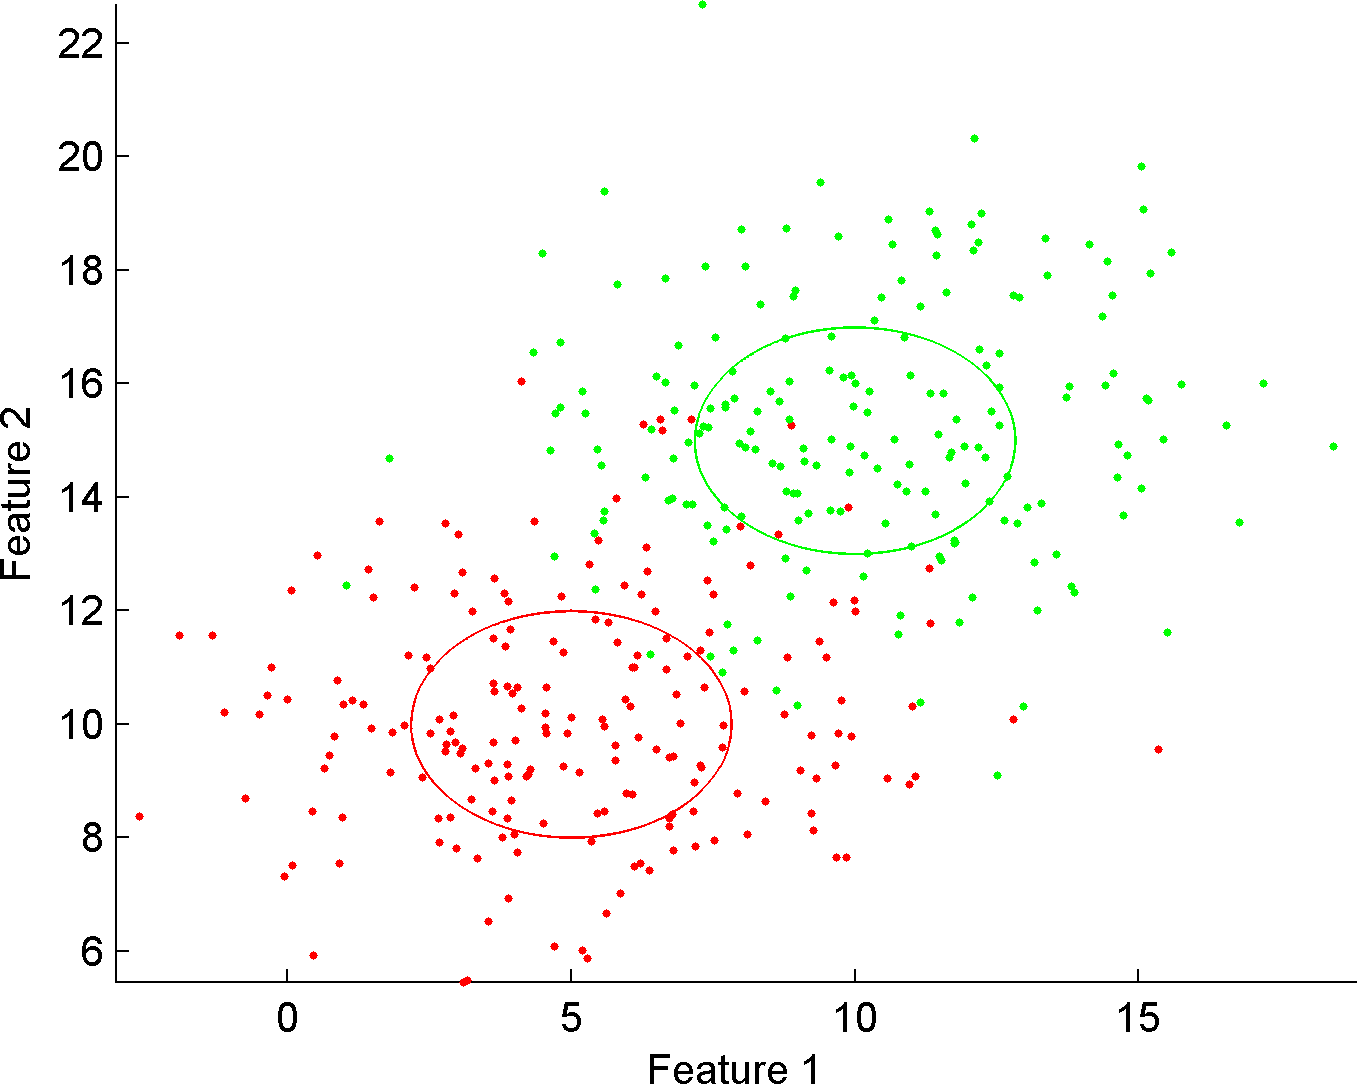
\includegraphics[width=0.9\linewidth]{fig1a-AB_cluster}
	\label{fig:clustersDataAB}
	\caption{Clusters A and B with unit standard deviation elipses}
\end{figure}

 \subsection{Classes C, D, E}
 The three classes C, D and E were characterized by:
 
 \begin{eqnarray}
{\mu}_{C}=\left[ \begin{smallmatrix} 5&10 \end{smallmatrix}\right]^{T} \; & {\Sigma}_{C}=\left[ \begin{smallmatrix} 8&4 \\ 4&40 \end{smallmatrix}\right]^{T} \nonumber\\
{\mu}_{D}=\left[ \begin{smallmatrix} 15&10 \end{smallmatrix}\right]^{T} \; & {\Sigma}_{D}=\left[ \begin{smallmatrix} 8&0 \\ 0&8 \end{smallmatrix}\right]^{T} \nonumber\\
{\mu}_{E}=\left[ \begin{smallmatrix} 10&5 \end{smallmatrix}\right]^{T} \; & {\Sigma}_{D}=\left[ \begin{smallmatrix} 10&-5 \\ -5&20 \end{smallmatrix}\right]^{T} \nonumber
\end{eqnarray}
 
 
\begin{figure}[ht]
\centering
	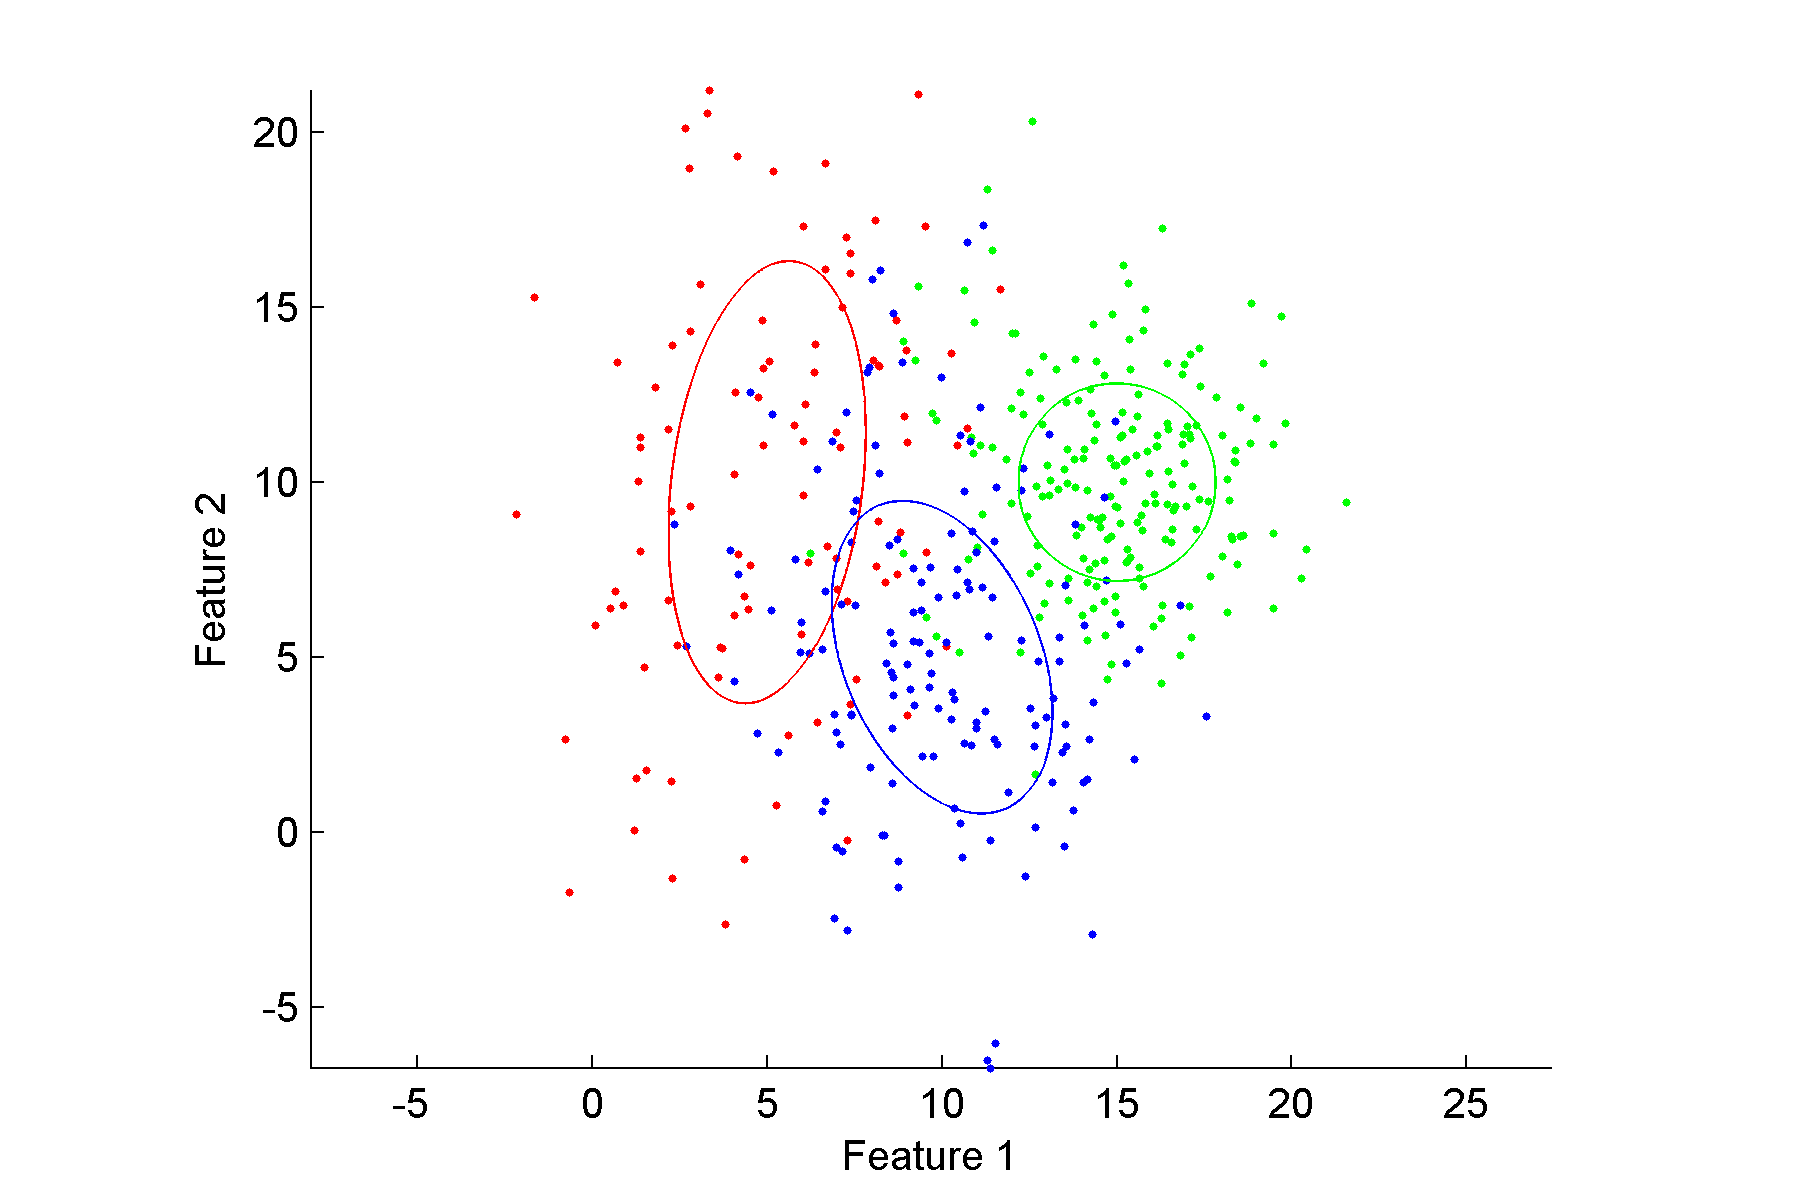
\includegraphics[width=0.9\linewidth]{fig1b-CDE_cluster}
	\label{fig:clustersDataCDE}
	\caption{Clusters C, D, E unit standard deviation elipses}
\end{figure}
 
\clearpage

\section{Classifiers}

\subsection{Implementation}

\subsubsection{Mean Euclidean Distance}

\subsubsection{General Euclidean Distance}
The GED classifier is implemented in a similar manner as the MED classifier. However, in the case of GED a whitening transform is applied to the samples to transform them onto a space where features are both uncorrelated, and have unit-variances. This is accomplished using the weighting matrix W. The distance between two points in the transformed space is calculated as,


\begin{eqnarray}
\label{eqn:GED-whitening}
\left [ W=\Lambda^{-1/2}\Phi^{T}  \right ]
\end{eqnarray}



In the above equation, $\Lambda$ contains the eigen values of the covariance matrix $\Sigma$ as elements, and $\Phi$ contains the eigenvectors of $\Sigma$. The simplified distance function is included in \ref{eqn:GED}.

\begin{eqnarray}
\label{eqn:GED}
{d}_{G}(x,z) = {\left [ (x-z)^{T}\Phi\Lambda^{-1/2}\Phi^{T}(x-z) \right ]}^{1/2}
\end{eqnarray}


The decision boundary is therefore calculated in the two- and three- class cases as,

\begin{eqnarray}
\label{eqn:boundary-GED}
& d_{E} (x,z_{1}) = d_{E} (x,z_{2}) \\
& \left [ (x-{z}_{1})^{T}\Phi\Lambda^{-1/2}\Phi^{T}(x-z_{1}) \right ]^{1/2} \\
= & \left [ (x-z_{2})^{T}\Phi\Lambda^{-1/2}\Phi^{T}(x-z_{2}) \right ]^{1/2}  \nonumber \\
&\left [ (x-{z}_{1})^{T}\Phi\Lambda^{-1/2}\Phi^{T}(x-z_{1}) \right ]^{1/2} \\
= &\left [ (x-z_{2})^{T}\Phi\Lambda^{-1/2}\Phi^{T}(x-z_{2}) \right ]^{1/2}  \nonumber \\
= &\left [ (x-z_{3})^{T}\Phi\Lambda^{-1/2}\Phi^{T}(x-z_{3}) \right ]^{1/2}  \nonumber
\end{eqnarray}



In the case of the MATLAB implementation, all points on the grid are classified based on identifying the minimum distance between the point and the mean of each class in the transformed space. This allows for a simple contour to be plotted showing the decision boundary between each class. This is shown below for both the two- and three- class case,

\begin{eqnarray}
\label{eqn:pointClass-GED}
min(d_{E} (x,z_{1}), d_{E} (x,z_{2})) \\
min(d_{E} (x,z_{1}), d_{E} (x,z_{2}), d_{E} (x,z_{3}))
\end{eqnarray}


This implementation of the GED classifier and method for creating the decision boundary is shown in Appendix A.

\subsubsection{Maximum A Posteriori}

\subsubsection{Nearest Neighbor}

The nearest neighbor classifier uses MATLAB implementation of $knnclassify$. A nearest neighbor classifier will test a point and compare its distance to all other known classified points. The test point will belong to the class which contains a point with the least Euclidian distance to the test point.

The classification boundary is constructed by evaluating many test points on a grid, using the generated data as training data. Due to the nature of nearest neighbor, all training data will be classified correctly; each classified point is its own nearest neighbor.

\subsubsection{Five Nearest Neighbor}

The 5NN classifier uses MATLAB implementation of $knnclassify$. A nearest neighbor classifier will test a point and compare its distance to all other known classified points. The 5 nearest classified points are determined, and the class of each of the points is determined. The class with the majority of class points in the 5 nearest neighbors is designated the class for the test point.

Note that the method of selecting the 5 nearest sample points from each class and selecting the class with the lowest sample mean was not used, as there exist many variations of the nearest neighbor method, and the MATLAB default is likely the default due to its accuracy.

The classification boundary is constructed by evaluating many test points on a grid, using the generated data as training data. Unlike nearest neighbor, 5 nearest neighbor will not classify all training data correctly; the use of 5 nearest neighbors means that not all points will have 2 other nearest neighbors that are of the same class.




\subsection{Results}
All classification methods were applied in each of Case 1 and Case 2. To apply the methods, the space of each case was divided into a 2-D array of discrete points whose range matched the range of the respective cluster data and whose resolution was equal to 0.05 along both feature axes. For each method and case, each point in the 2-D array was classified. MATLAB's $contour()$ was used with each 2-D array to produce the classifier boundaries.

To aid in analysis, MED, GED, and MAP classifier boundaries are all plotted together in one figure, along with data clusters and unit standard deviation contours. In the Case 1 scenario (Figure~\ref{fig:med_ged_map_classifier_case1}), the GED and MAP classification boundaries, shown as magenta and blue lines respectively, lie on top of each other with the magenta line being obscured. This is because the MAP classifier is reduced to GED in this case, as the a priori probabilities for each class are equal. The classification boundaries are essentially two very slightly curved, but relatively straight, lines separating the two data clusters. The MED classification boundary is represented by the steeper straight cyan line. This makes sense intuitively, as the classification boundary represents the perpendicular bisector of the mean in each cluster. In the MED case only the mean, and not the covariance information for the two classes, is considered.

\begin{figure}[ht]
\centering
	{
	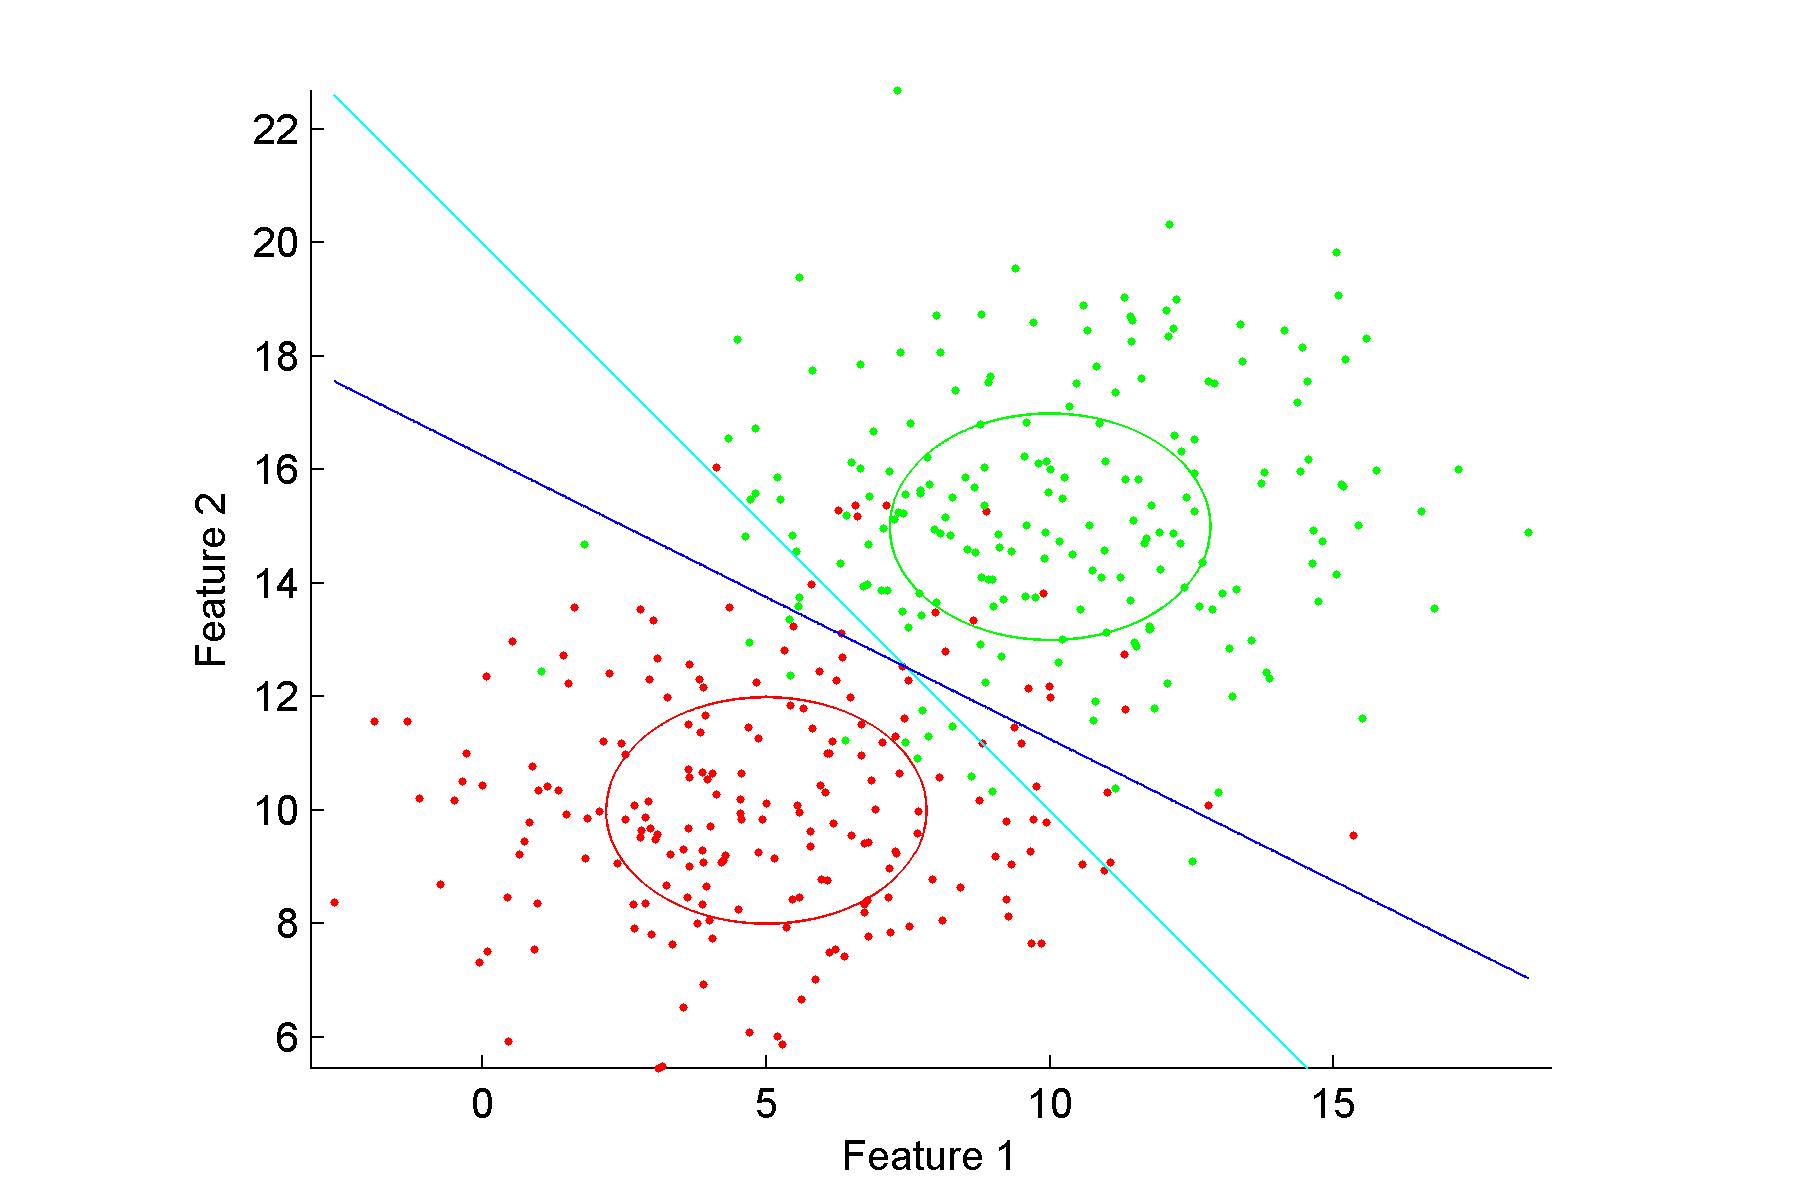
\includegraphics[width=0.45\linewidth]{fig2a-AB_MED_MICD_MAP}
	}
	
	\caption{MED, GED, and MAP classification boundaries for Case 1}
	\label{fig:med_ged_map_classifier_case1}
\end{figure}

In the Case 2 scenario (Figure~\ref{fig:med_ged_map_classifier_case2}), the MED classification boundary is shown as the light blue lines. The MED classification boundary is shown to be three straight lines, interescting near the mid-point between the three data clusters. The MED classifier does not take into account the covariance matrices of the three data clusters, so the performance described is as expected. The GED classification boundary is shown as the contoured magenta lines in the figure, intersecting near the midpoint between the three classes of data. This is an intuitive result, as the classification boundary better wraps around the unit standard deviation contours for three data classes. The MAP decision boundary is shown as the blue lines, slightly offset to the left of the GED decision boundary. In this case the decision boundaries do not overlay each other as in the Case 1 scenario. This is a result of the a priori probabilities for each of the three classes being different in this case, with the probability information altering the performance of the classification method.

\begin{figure}[ht]
\centering
	{
	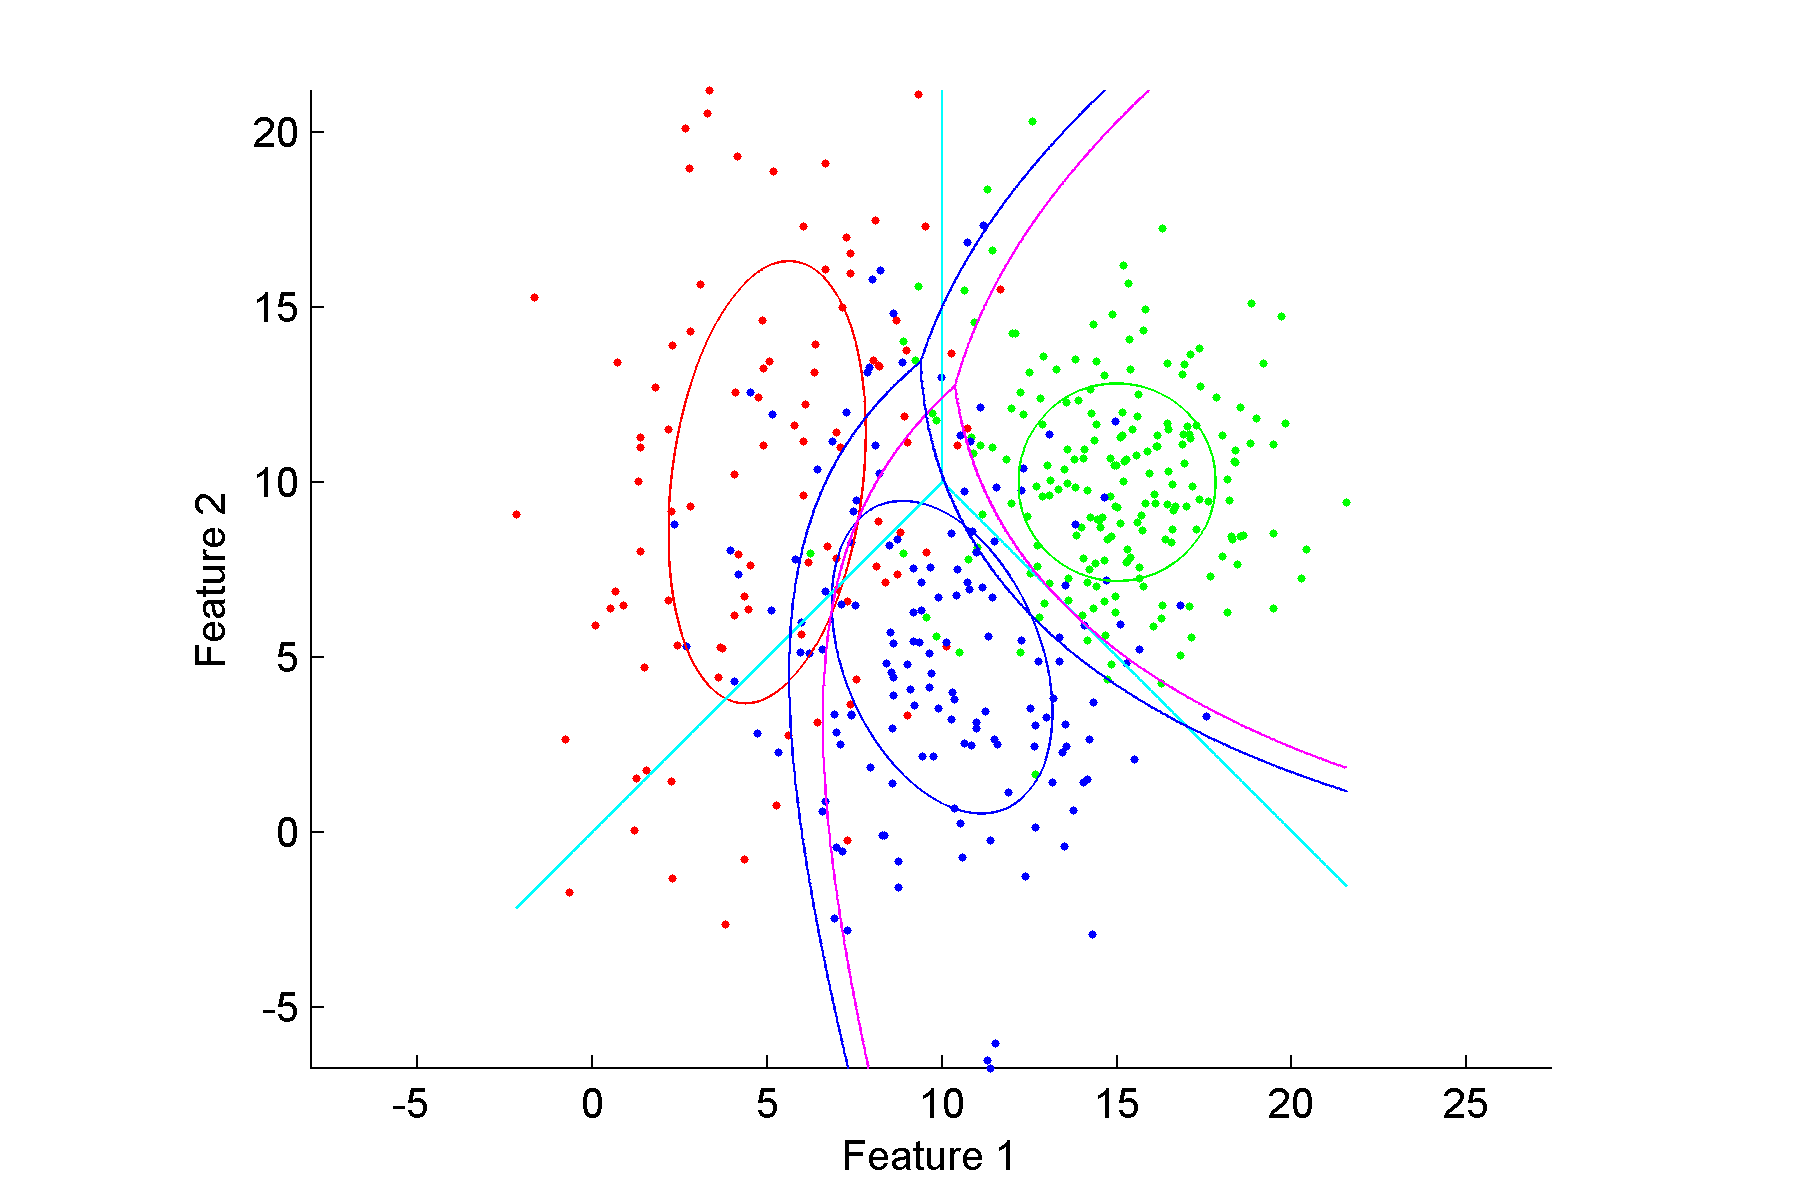
\includegraphics[width=0.45\linewidth]{fig2b-AB_MED_MICD_MAP}
	}
	
	\caption{MED, GED, and MAP classification boundaries for Case 2}
	\label{fig:med_ged_map_classifier_case2}
\end{figure}

Next, the NN and 5NN classification boundaries were plotted together for both the Case 1 and Case 2 data sets, along with unit variance contours for each class, to allow for comparison. The decision boundaries for Case 1 (Figure~\ref{fig:nn_boundary_case1}) are fairly similar for both methods, with the decision boundaries being shown as jagged lines separating the data. The key difference in the two methods is that the 5NN classification method does not result in classification boundaries around outliers of the two data sets.

\begin{figure}[ht]
\centering
	\subfigure[NN classification for Case 1]{
	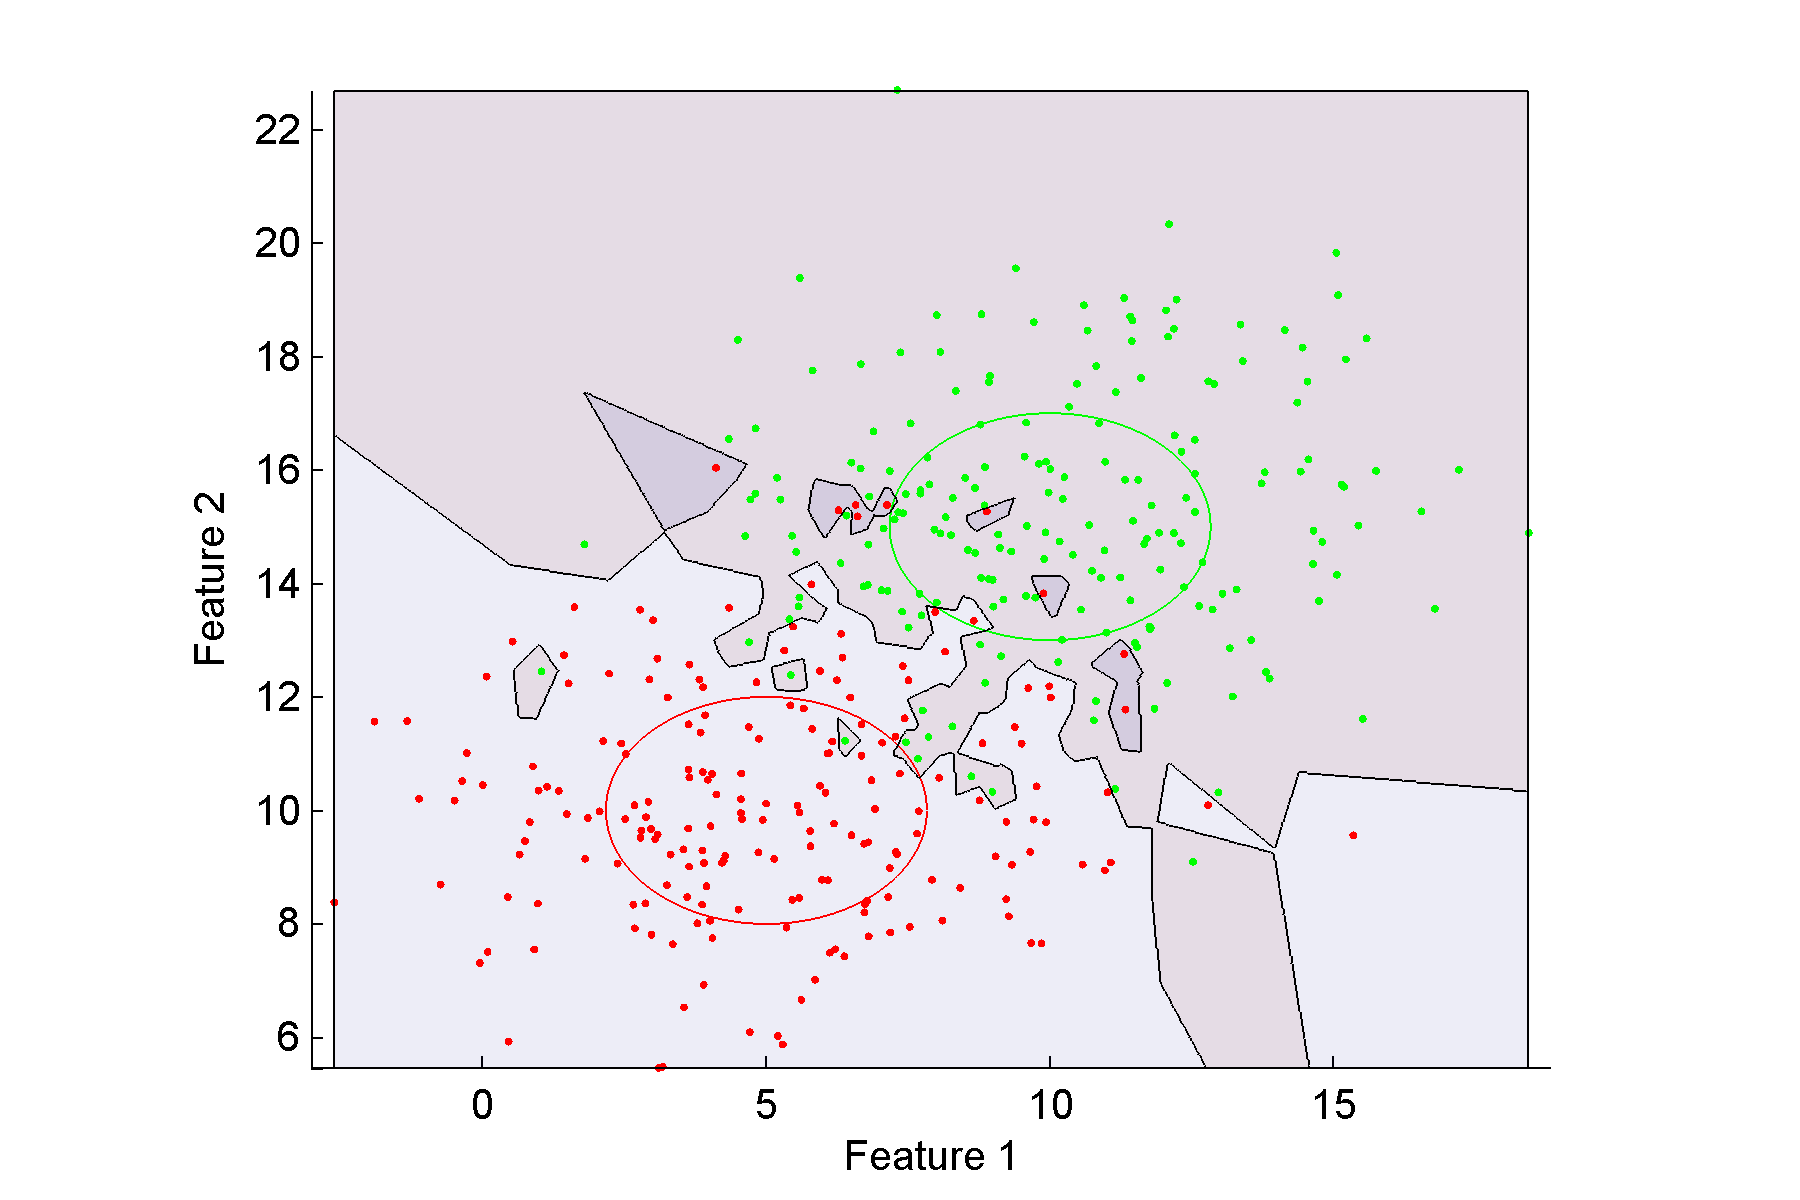
\includegraphics[width=0.45\linewidth]{fig3a-AB_NN}
	}
	\subfigure[5NN classification for Case 1]{
	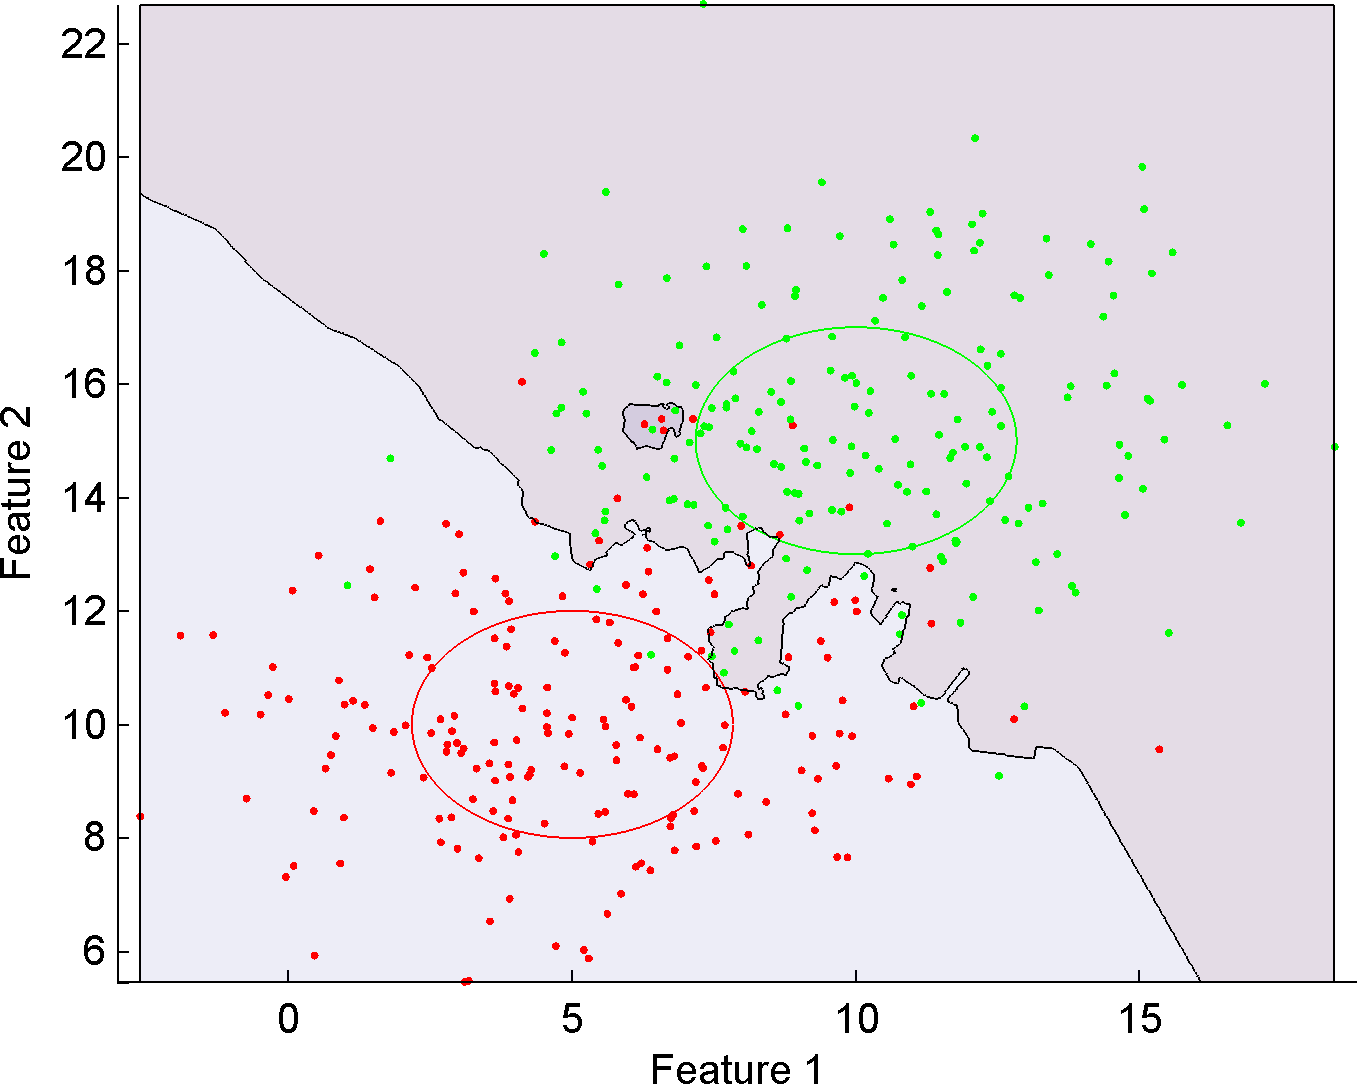
\includegraphics[width=0.45\linewidth]{fig4a-AB_5NN}
	}
	
	\caption{Nearest Neighbor boundaries for Case 1}
	\label{fig:nn_boundary_case1}
\end{figure}

For the Case 2 scenario (Figure~\ref{fig:nn_boundary_case2}), performance of the two methods was similar. Again, the sensitivity of the NN method to outliers is seen to result to decision boundaries encircling outliers. The 5NN classifier is not as prone to these outliers, resulting in a more intuitive decision boundary between the three classes of data.

\begin{figure}[ht]
\centering
	\subfigure[NN classification for Case 2]{
	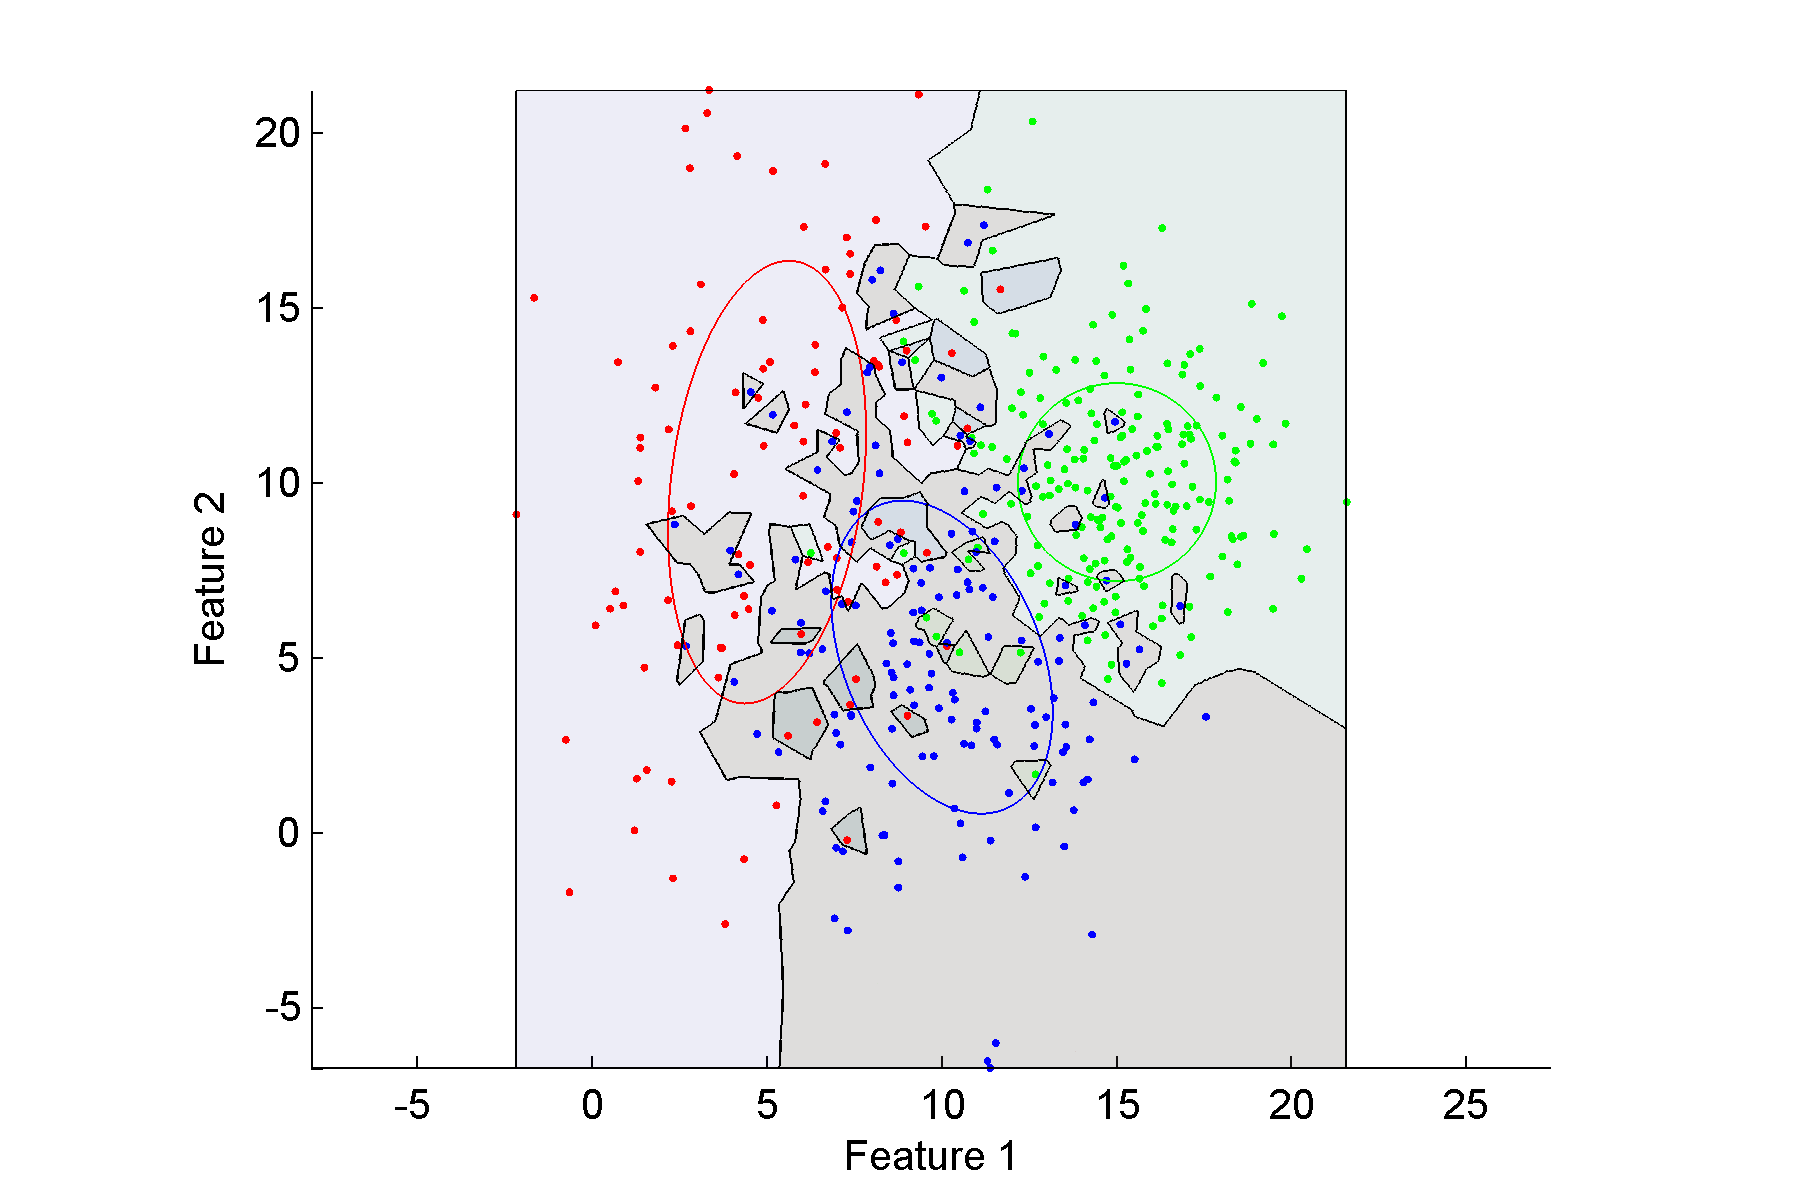
\includegraphics[width=0.45\linewidth]{fig3b-CDE_NN}
	}
	\subfigure[5NN classification for Case 2]{
	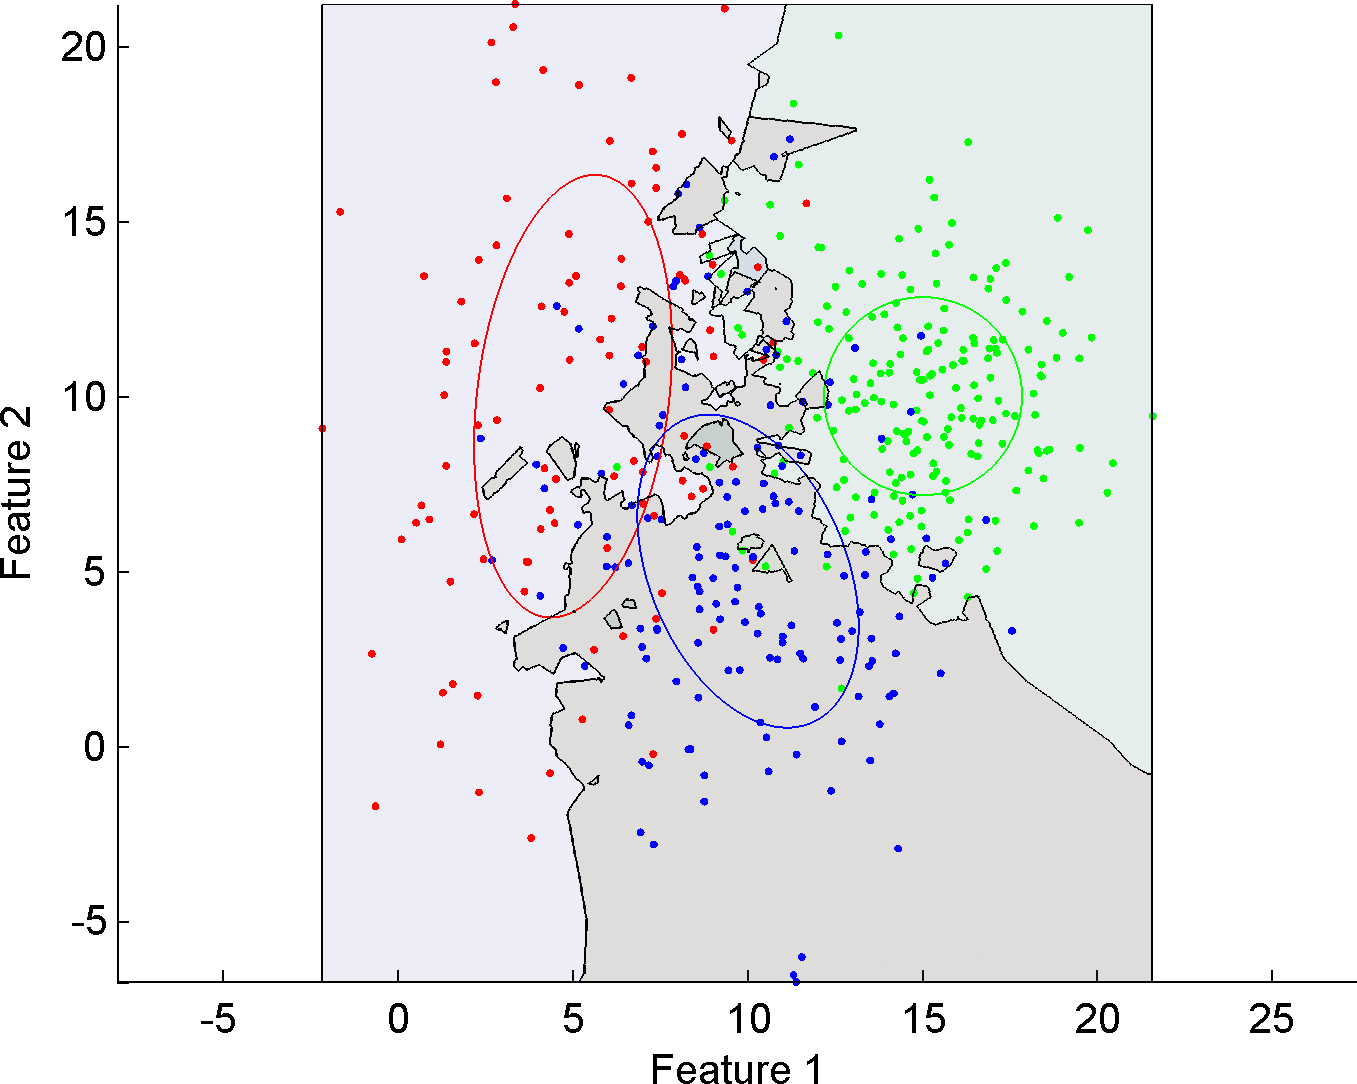
\includegraphics[width=0.45\linewidth]{fig4b-CDE_5NN}
	}
	
	\caption{Nearest Neighbor boundaries for Case 2}
	\label{fig:nn_boundary_case2}
\end{figure}

\section{Error Analysis}
\subsection{Experimental error rate}
To find the experimental error rate $P(\epsilon)$ for Case 1, a discretized form of the following equation was used.
\begin{eqnarray}
\label{eqn:2-class_cont_PofE}
P(\epsilon)=\int_{R_A}P(\underbar {x}|B)P(B)d\underbar {x} +
            \int_{R_B}P(\underbar {x}|A)P(A)d\underbar {x}
\end{eqnarray}

The discretized form becomes
\begin{eqnarray}
\label{eqn:2-class_disc_PofE}
P(\epsilon)\approx\sum_{i,j\ in\ R_A}P(\underbar {x}|B)_{i,j}P(B)wh +
                  \sum_{i.j\ in\ R_B}P(\underbar {x}|A)_{i,j}P(A)wh
\end{eqnarray}

where $w$ and $l$ are the width and height of the discretized points. The MAP classification boundary that were found previously were used for determining $R_A$ and $R_B$. Although the equation describes summing values over an infinite number of points, a finite set of points had to be selected to feasibly perform the calculation. This introduces some negligible error. The same number of points used to calculate the classification data was used to calculate $P(\epsilon)$. The result was $P(\epsilon)\approx0.06281$.

To find $P(\epsilon)$ for Case 2, the same method was used as in Case 1 except that the equation for $P(\epsilon)$ had to be modified for three classes.
\begin{eqnarray}
\label{eqn:3-class_cont_PofE}
P(\epsilon)& = \int_{R_C}[P(\underbar{x}|D)P(D)+P(\underbar{x}|E)P(E)]d\underbar{x} \\
           & + \int_{R_D}[P(\underbar{x}|C)P(C)+P(\underbar{x}|E)P(E)]d\underbar{x} \nonumber\\
           & + \int_{R_E}[P(\underbar{x}|C)P(C)+P(\underbar{x}|D)P(D)]d\underbar{x}\nonumber
\end{eqnarray}

The discretized form of this equation becomes
\begin{eqnarray}
\label{eqn:3-class_disc_PofE}
P(\epsilon)&\approx \sum_{i,j\ in\ R_C}[P(\underbar{x}|D)_{i,j}P(D)+P(\underbar{x}|E)_{i,j}P(E)]wh \\
           & +      \sum_{i,j\ in\ R_D}[P(\underbar{x}|C)_{i,j}P(C)+P(\underbar{x}|E)_{i,j}P(E)]wh \nonumber\\
           & +      \sum_{i,j\ in\ R_E}[P(\underbar{x}|C)_{i,j}P(C)+P(\underbar{x}|D)_{i,j}P(D)]wh \nonumber
\end{eqnarray}

The result for Case 2 was found to be $P(\epsilon)\approx0.1686$.

Case 1 was found to have a much lower experimental error rate than Case 2. This was expected because Case 2 had one more class than Case 1 and because the unit standard deviation contours of the clusters of Case 2 were much closer together than the contours of the clusers of Case 1.
 
\subsection{Confusion matrices for GED, MED and MAP}

A confusion matrix shows the performance of a classifier on a set of data. It compares the true values of the data against the predicted classifications by the classifier, and attempts to quantify the types of errors being made.

For the GED, MED and MAP classifiers, the same data used to generate the classifier was used to test the classifier.

\subsubsection{GED}
\begin{figure}[!ht]
\begin{minipage}[b]{0.5\linewidth}
\centering
	\begin{tabular}{ccc|c|c}
	 & &\multicolumn{2}{c}{Predicted} &\\
	  & & \bf{A} &  \bf{B} & total \\
	 \cline{3-5}
	 \multirow{2}{*}{\begin{sideways}Actual\end{sideways}} & \bf{A'}& 186 & 14 & 200 \\
	 \cline{3-5}
	 & \bf{B'}& 10 & 190 & 200 \\
	  \cline{3-5}
	 &total&196&204&\\
	\end{tabular}
\end{minipage}
\hspace{0.5cm}
\begin{minipage}[b]{0.5\linewidth}
	\begin{tabular}{r|c}
	\hline
	Correct& 376\\
	Total& 400\\
	\hline
	\% Correct& 94\%\\
	\hline
	\end{tabular}
\end{minipage}
\vspace{1mm}
\caption{GED performance on A and B}
\end{figure}

\begin{figure}[!ht]
\begin{minipage}[b]{0.5\linewidth}
\centering
	\begin{tabular}{ccc|c|c|c}
	 & &\multicolumn{3}{c}{Predicted} &\\
	  & & \bf{C} &  \bf{D} & \bf{E} & total \\
	 \cline{3-6}
	 \multirow{3}{*}{\begin{sideways}Actual\end{sideways}} & \bf{C'}& 91 & 0 & 9 & 100\\
	 \cline{3-6}
	 & \bf{D'}& 6 & 164 & 30 & 200\\
	  \cline{3-6}
	 & \bf{E'}& 29 & 11 & 110 &  150\\
	  \cline{3-6}
	 &total&126&175&149\\
	\end{tabular}
\end{minipage}
\hspace{0.5cm}
\begin{minipage}[b]{0.5\linewidth}
	\begin{tabular}{r|c}
	\hline
	Correct& 365\\
	Total& 450\\
	\hline
	\% Correct& 81.1\%\\
	\hline
	\end{tabular}
\end{minipage}
\vspace{1mm}
\caption{GED performance on C, D and E}
\end{figure}

\clearpage

\subsubsection{MED}
\begin{figure}[!ht]
\begin{minipage}[b]{0.5\linewidth}
\centering
	\begin{tabular}{ccc|c|c}
	 & &\multicolumn{2}{c}{Predicted} &\\
	  & & \bf{A} &  \bf{B} & total \\
	 \cline{3-5}
	 \multirow{2}{*}{\begin{sideways}Actual\end{sideways}} & \bf{A'}& 184 & 16 & 200 \\
	 \cline{3-5}
	 & \bf{B'}& 10 & 190 & 200 \\
	  \cline{3-5}
	 &total&196&204&\\
	\end{tabular}
\end{minipage}
\hspace{0.5cm}
\begin{minipage}[b]{0.5\linewidth}
	\begin{tabular}{r|c}
	\hline
	Correct& 374\\
	Total& 400\\
	\hline
	\% Correct& 93.5\%\\
	\hline
	\end{tabular}
\end{minipage}
\vspace{1mm}
\caption{MED performance on A and B}
\end{figure}


\begin{figure}[!ht]
\begin{minipage}[b]{0.5\linewidth}
\centering
	\begin{tabular}{ccc|c|c|c}
	 & &\multicolumn{3}{c}{Predicted} &\\
	  & & \bf{C} &  \bf{D} & \bf{E} & total \\
	 \cline{3-6}
	 \multirow{3}{*}{\begin{sideways}Actual\end{sideways}} & \bf{C'}& 70 & 1 & 29 & 100\\
	 \cline{3-6}
	 & \bf{D'}& 9 & 167 & 24 & 200\\
	  \cline{3-6}
	 & \bf{E'}& 27 & 13 & 110 &  150\\
	  \cline{3-6}
	 &total&106&181&163\\
	\end{tabular}
\end{minipage}
\hspace{0.5cm}
\begin{minipage}[b]{0.5\linewidth}
	\begin{tabular}{r|c}
	\hline
	Correct& 347\\
	Total& 450\\
	\hline
	\% Correct& 77.1\%\\
	\hline
	\end{tabular}
\end{minipage}
\vspace{1mm}
\caption{MED performance on C, D and E}
\end{figure}

\subsubsection{MAP}
\begin{figure}[!ht]
\begin{minipage}[b]{0.5\linewidth}
\centering
	\begin{tabular}{ccc|c|c}
	 & &\multicolumn{2}{c}{Predicted} &\\
	  & & \bf{A} &  \bf{B} & total \\
	 \cline{3-5}
	 \multirow{2}{*}{\begin{sideways}Actual\end{sideways}} & \bf{A'}& 186 & 14 & 200 \\
	 \cline{3-5}
	 & \bf{B'}& 10 & 190 & 200 \\
	  \cline{3-5}
	 &total&196&204&\\
	\end{tabular}
\end{minipage}
\hspace{0.5cm}
\begin{minipage}[b]{0.5\linewidth}
	\begin{tabular}{r|c}
	\hline
	Correct& 376\\
	Total& 400\\
	\hline
	\% Correct& 94\%\\
	\hline
	\end{tabular}
\end{minipage}
\vspace{1mm}
\caption{MAP performance on A and B}
\end{figure}


\begin{figure}[!ht]
\begin{minipage}[b]{0.5\linewidth}
\centering
	\begin{tabular}{ccc|c|c|c}
	 & &\multicolumn{3}{c}{Predicted} &\\
	  & & \bf{C} &  \bf{D} & \bf{E} & total \\
	 \cline{3-6}
	 \multirow{3}{*}{\begin{sideways}Actual\end{sideways}} & \bf{C'}& 79 & 0 & 21 & 100\\
	 \cline{3-6}
	 & \bf{D'}& 4 & 174 & 22 & 200\\
	  \cline{3-6}
	 & \bf{E'}& 23 & 20 & 107 &  150\\
	  \cline{3-6}
	 &total&106&194&150\\
	\end{tabular}
\end{minipage}
\hspace{0.5cm}
\begin{minipage}[b]{0.5\linewidth}
	\begin{tabular}{r|c}
	\hline
	Correct& 360\\
	Total& 450\\
	\hline
	\% Correct& 80\%\\
	\hline
	\end{tabular}
\end{minipage}
\vspace{1mm}
\caption{MAP performance on C, D and E}
\end{figure}

\clearpage

\subsection{NN and 5NN}

For the NN and 5NN classifiers, the classifiers were developed from a set of training data, and the classifier was tested with a new set of data, distributed with the same underlying statistics as the training data. This data set was of the same size as the training data set.

\subsubsection{NN}
\begin{figure}[!ht]
\begin{minipage}[b]{0.5\linewidth}
\centering
	\begin{tabular}{ccc|c|c}
	 & &\multicolumn{2}{c}{Predicted} &\\
	  & & \bf{A} &  \bf{B} & total \\
	 \cline{3-5}
	 \multirow{2}{*}{\begin{sideways}Actual\end{sideways}} & \bf{A'}& 83 & 17 & 100 \\
	 \cline{3-5}
	 & \bf{B'}& 21 & 179 & 200 \\
	  \cline{3-5}
	 &total&104&196&\\
	\end{tabular}
\end{minipage}
\hspace{0.5cm}
\begin{minipage}[b]{0.5\linewidth}
	\begin{tabular}{r|c}
	\hline
	Correct& 279\\
	Total& 400\\
	\hline
	\% Correct& 69.8\%\\
	\hline
	\end{tabular}
\end{minipage}
\vspace{1mm}
\caption{Nearest Neighbour performance on A and B}
\end{figure}


\begin{figure}[!ht]
\begin{minipage}[b]{0.5\linewidth}
\centering
	\begin{tabular}{ccc|c|c|c}
	 & &\multicolumn{3}{c}{Predicted} &\\
	  & & \bf{C} &  \bf{D} & \bf{E} & total \\
	 \cline{3-6}
	 \multirow{3}{*}{\begin{sideways}Actual\end{sideways}} & \bf{C'}& 63 & 2 & 35 & 100\\
	 \cline{3-6}
	 & \bf{D'}& 3 & 160 & 37 & 200\\
	  \cline{3-6}
	 & \bf{E'}& 20 & 28 & 102 &  150\\
	  \cline{3-6}
	 &total&86&190&141\\
	\end{tabular}
\end{minipage}
\hspace{0.5cm}
\begin{minipage}[b]{0.5\linewidth}
	\begin{tabular}{r|c}
	\hline
	Correct& 325\\
	Total& 450 \\
	\hline
	\% Correct& 72.2\%\\
	\hline
	\end{tabular}
\end{minipage}
\vspace{1mm}
\caption{Nearest Neighbour performance on C, D and E}
\end{figure}

\clearpage

\subsubsection{5NN}
\begin{figure}[!ht]
\begin{minipage}[b]{0.5\linewidth}
\centering
	\begin{tabular}{ccc|c|c}
	 & &\multicolumn{2}{c}{Predicted} &\\
	  & & \bf{A} &  \bf{B} & total \\
	 \cline{3-5}
	 \multirow{2}{*}{\begin{sideways}Actual\end{sideways}} & \bf{A'}& 94 & 6 & 100 \\
	 \cline{3-5}
	 & \bf{B'}& 34 & 166 & 200 \\
	  \cline{3-5}
	 &total&128&172\\
	\end{tabular}
\end{minipage}
\hspace{0.5cm}
\begin{minipage}[b]{0.5\linewidth}
	\begin{tabular}{r|c}
	\hline
	Correct& 260\\
	Total& 300\\
	\hline
	\% Correct& 86.7\%\\
	\hline
	\end{tabular}
\end{minipage}
\vspace{1mm}
\caption{5 Nearest Neighbour performance on A and B}
\end{figure}

	
\begin{figure}[!ht]
\begin{minipage}[b]{0.5\linewidth}
\centering
	\begin{tabular}{ccc|c|c|c}
	 & &\multicolumn{3}{c}{Predicted} &\\
	  & & \bf{C} &  \bf{D} & \bf{E} & total \\
	 \cline{3-6}
	 \multirow{3}{*}{\begin{sideways}Actual\end{sideways}} & \bf{C'}& 75 & 0 & 25 & 100\\
	 \cline{3-6}
	 & \bf{D'}& 1 & 181 & 18 & 200\\
	  \cline{3-6}
	 & \bf{E'}& 14 & 24 & 112 &  150\\
	  \cline{3-6}
	 &total&90&205&155\\
	\end{tabular}
\end{minipage}
\hspace{0.5cm}
\begin{minipage}[b]{0.5\linewidth}
	\begin{tabular}{r|c}
	\hline
	Correct& 368\\
	Total& 450\\
	\hline
	\% Correct& 81.8\%\\
	\hline
	\end{tabular}
\end{minipage}
\vspace{1mm}
\caption{5 Nearest Neighbour performance on C, D and E}
\end{figure}

The confusion matrices of Case 2 show that points that actually belong to cluster E are the least likely to be classified correctly. Similar to why the experimental error rate for Case 2 was lower than Case 1, the greater difficulty in correctly classifying points of cluster E is because of how close cluster E is to the other two clusters. Cluster E is partially between clusters C and D. The GED and MAP classifier boundaries show this close proximity very well.
 
\clearpage


\section{Conclusions}
Implementation of five classifiers (MED, GED, MAP, NN, and 5NN) in MATLAB was used to analyze the performance of each classifier. First, each method was implemented and used to classify a two-class and three-class data set. The classifiers were used to determine decision boundaries in each case, resulting in some initial observations about model performance. Overall, MED performed poorly, with GED and MAP classifiers performing significantly better. It was also seen that the 5NN classifier outperformed the NN classifier in rejecting statistical outliers in the data.

As noted in the earlier error analysis, MAP outperformed the MED, GED, NN, and 5NN classifiers in the scenario of Case 1. This is because MAP inherently attempts to minimize the probability of error, resulting in it outperforming other classifiers in terms of probability of error. MED does not consider the probability of error, or the the covariance of the data, and therefore performs relatively poorly. GED performs significantly better than MED for Case 1, and almost performs at the level of the MAP classifier. This is because GED considers the covariance of each class of data, though unlike MAP it does not consider the probability of error. The NN and 5NN classifiers are markedly outperformed by the other techniques, a result of them poorly classifying the new set of test data.

In the scenario of Case 2 the probability of error increased significantly for all classifiers. However, the same trend of MAP outperforming GED and MED, and GED outperforming MED, was conserved. It is notable in this case, however, that the performance of the NN and 5NN classifiers was competitive with other methods. The 5NN method still performed better than the NN method, due to it's ability to reject outliers. The improvement in performance of the 5NN and NN techniques here is likely due to both methods being able to account for the number of data points in each class and adjust accordingly - something the other classifiers are unable to accomplish.


\appendix
\newpage

\section{Matlab Code}
\subsection{PSNR function}
%\lstinputlisting[language=Matlab]{"matlabFiles/psnr.m"}

\subsection{Chroma Subsampling}
%\lstinputlisting[language=Matlab]{"matlabFiles/lab3_q2.m"}

\subsection{Image Transform}
%\lstinputlisting[language=Matlab]{"matlabFiles/lab3_q3.m"}

\subsection{Quantization}
%\lstinputlisting[language=Matlab]{"matlabFiles/lab3_q2.m"}






% -------- Bibliography --------
%\addcontentsline{toc}{chapter}{\hspace{13pt} References}
\bibliography{refs}

\end{document}  
